%
% discontinuities.tex -- 
%
% (c) 2019 Prof Dr Andreas Mueller
%
\section{Propagation of discontinuities}
\rhead{Discontinuities}
The study of the wave equation at the beginning of this chapter
allowed us to find solutions as translates of an initial function
$u_0$ along the characteristics, which were straight lines
$x\pm at=\operatorname{const}$.
If $u_0$ is not everywhere differentiable, then the solution will
not be differentiable along the characteristic.

Assume that $u$ is continuously differentiable everywhere
and twice continuously differentiable everywhere
except along a curve.
This curve separates the domain into to subdomains.
In each subdomain, $u$ is a solution of the differential equation
with the same boundary values and tangent planes on the curve.
This implies that the curve and the tangent planes must
specify a characteristic strip.

\begin{satz}
If $u$ is continuously differentiable everywhere and twice
continuously differentiable everywhere except along a curve,
and $u$ is a solution everywhere except on that curve,
then that curve is a characteristic.
\end{satz}

This means that discontinuities of the second derivative
can only propagate along the characteristic curves.

The wave equation can be used to approximately compute the
flow around a supersonic plane.
The plane produces shock waves which are discontinuities in the
solution of the wave equation.
According to the theorem above, these shock waves follow
characteristic curves.
The can be made visible using the Schlieren technique
(figure~\ref{ueberschall2d}).

\begin{figure}
\begin{center}
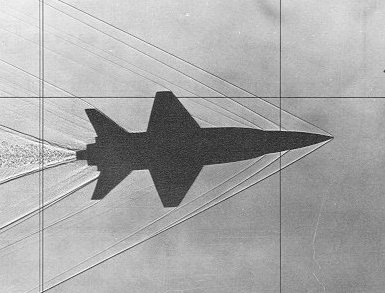
\includegraphics[width=0.8\hsize]{../common/graphics/i-5-1}
\end{center}
\caption{Flow around a supersonic plane\label{ueberschall2d}}
\end{figure}

